% This is "sig-alternate.tex" V2.1 April 2013
% This file should be compiled with V2.5 of "sig-alternate.cls" May 2012
%
% This example file demonstrates the use of the 'sig-alternate.cls'
% V2.5 LaTeX2e document class file. It is for those submitting
% articles to ACM Conference Proceedings WHO DO NOT WISH TO
% STRICTLY ADHERE TO THE SIGS (PUBS-BOARD-ENDORSED) STYLE.
% The 'sig-alternate.cls' file will produce a similar-looking,
% albeit, 'tighter' paper resulting in, invariably, fewer pages.
%
% --------------------------------------------------------------
% This .tex file (and associated .cls V2.5) produces:
%       1) The Permission Statement
%       2) The Conference (location) Info information
%       3) The Copyright Line with ACM data
%       4) NO page numbers
%
% as against the acm_proc_article-sp.cls file which
% DOES NOT produce 1) thru' 3) above.
%
% Using 'sig-alternate.cls' you have control, however, from within
% the source .tex file, over both the CopyrightYear
% (defaulted to 200X) and the ACM Copyright Data
% (defaulted to X-XXXXX-XX-X/XX/XX).
% e.g.
% \CopyrightYear{2007} will cause 2007 to appear in the copyright line.
% \crdata{0-12345-67-8/90/12} will cause 0-12345-67-8/90/12 to appear in the copyright line.
%
% ---------------------------------------------------------------------------
% This .tex source is an example which *does* use
% the .bib file (from which the .bbl file % is produced).
% REMEMBER HOWEVER: After having produced the .bbl file,
% and prior to final submission, you *NEED* to 'insert'
% your .bbl file into your source .tex file so as to provide
% ONE 'self-contained' source file.
%
% ================= IF YOU HAVE QUESTIONS =======================
% Questions regarding the SIGS styles, SIGS policies and
% procedures, Conferences etc. should be sent to
% Adrienne Griscti (griscti@acm.org)
%
% Technical questions _only_ to
% Gerald Murray (murray@hq.acm.org)
% ===============================================================
%
% For tracking purposes - this is V2.0 - May 2012

\documentclass{sig-alternate}

\usepackage{longtable}
\usepackage{tabu}
\usepackage{multirow}

%\usepackage[hyphens]{url}
\usepackage{rotating}
\usepackage{underscore}

\usepackage{booktabs}
\usepackage[table]{xcolor}
\definecolor{Gray}{gray}{0.9}

\usepackage{todonotes}

\newcommand{\definition}[1]{\textit{#1}}

\begin{document}

% Copyright
\setcopyright{acmcopyright}
%\setcopyright{acmlicensed}
%\setcopyright{rightsretained}
%\setcopyright{usgov}
%\setcopyright{usgovmixed}
%\setcopyright{cagov}
%\setcopyright{cagovmixed}



% DOI
\doi{10.475/123_4}

% ISBN
\isbn{123-4567-24-567/08/06}



\acmPrice{\$15.00}

%
% --- Author Metadata here ---
%Conference
\conferenceinfo{GECCO'16,} {July 20-24, 2016, Denver, Colorado, USA.}
\CopyrightYear{2016}
\crdata{TBA}
\clubpenalty=10000
\widowpenalty = 10000
% --- End of Author Metadata ---

\title{The Impact of Hyperselection on Lexicase Selection}

%\subtitle{[Extended Abstract]}
%
% You need the command \numberofauthors to handle the 'placement
% and alignment' of the authors beneath the title.
%
% For aesthetic reasons, we recommend 'three authors at a time'
% i.e. three 'name/affiliation blocks' be placed beneath the title.
%
% NOTE: You are NOT restricted in how many 'rows' of
% "name/affiliations" may appear. We just ask that you restrict
% the number of 'columns' to three.
%
% Because of the available 'opening page real-estate'
% we ask you to refrain from putting more than six authors
% (two rows with three columns) beneath the article title.
% More than six makes the first-page appear very cluttered indeed.
%
% Use the \alignauthor commands to handle the names
% and affiliations for an 'aesthetic maximum' of six authors.
% Add names, affiliations, addresses for
% the seventh etc. author(s) as the argument for the
% \additionalauthors command.
% These 'additional authors' will be output/set for you
% without further effort on your part as the last section in
% the body of your article BEFORE References or any Appendices.

\numberofauthors{3} %  in this sample file, there are a *total*
% of EIGHT authors. SIX appear on the 'first-page' (for formatting
% reasons) and the remaining two appear in the \additionalauthors section.
%
\author{
% You can go ahead and credit any number of authors here,
% e.g. one 'row of three' or two rows (consisting of one row of three
% and a second row of one, two or three).
%
% The command \alignauthor (no curly braces needed) should
% precede each author name, affiliation/snail-mail address and
% e-mail address. Additionally, tag each line of
% affiliation/address with \affaddr, and tag the
% e-mail address with \email.
%
% 1st. author
\alignauthor
Author omitted\\
       \affaddr{.}\\
       \affaddr{.}\\
       \affaddr{.}\\
       \email{.}
% 2nd. author
\alignauthor
Author omitted\\
       \affaddr{.}\\
       \affaddr{.}\\
       \affaddr{.}\\
       \email{.}
% 3rd. author
\alignauthor
Author omitted\\
       \affaddr{.}\\
       \affaddr{.}\\
       \affaddr{.}\\
       \email{.}
}

% Just remember to make sure that the TOTAL number of authors
% is the number that will appear on the first page PLUS the
% number that will appear in the \additionalauthors section.

\maketitle
\begin{abstract}

Lexicase selection is a parent selection method that can improve the problem solving power of genetic programming. Previous work has shown that it can also produce \emph{hyperselection} events, in which a single individual is selected many more times than is possible under other selection methods. Here we investigate the role that hyperselection plays in the problem-solving performance of lexicase selection. We conduct runs of genetic programming on a set of software synthesis benchmark problems using lexicase and tournament selection, confirming that hyperselection occurs only with the former, which also performs significantly better. We then introduce a new \emph{sampled lexicase-tournament selection} method, which chooses individuals from a pool produced by lexicase selection, but with frequencies similar to those of tournament selection. If hyperselection is responsible for the problem-solving performance of lexicase selection, then sampled lexicase-tournament selection should not perform as well as lexicase selection. Additional runs show that sampled lexicase-tournament selection does perform comparably to lexicase selection. We conclude that the power of lexicase selection stems from the collection of individuals that it selects, not from the unusual frequencies with which it sometimes selects them.

\end{abstract}


%
% The code below should be generated by the tool at
% http://dl.acm.org/ccs.cfm
% Please copy and paste the code instead of the example below. 
%
\begin{CCSXML}
	<ccs2012>
	<concept>
	<concept_id>10010147.10010178.10010205.10010206</concept_id>
	<concept_desc>Computing methodologies~Heuristic function construction</concept_desc>
	<concept_significance>500</concept_significance>
	</concept>
	<concept>
	<concept_id>10010147.10010257.10010293.10011809.10011813</concept_id>
	<concept_desc>Computing methodologies~Genetic programming</concept_desc>
	<concept_significance>500</concept_significance>
	</concept>
	</ccs2012>
\end{CCSXML}

\ccsdesc[500]{Computing methodologies~Heuristic function construction}
\ccsdesc[500]{Computing methodologies~Genetic programming}

%
% End generated code
%

%
%  Use this command to print the description
%
\printccsdesc

% We no longer use \terms command
%\terms{Theory}

\keywords{Hyperselection, lexicase selection, software synthesis, tournament selection}

\section{Introduction}
\label{section:introduction}

Evolutionary computation systems use selection to direct search, with the goal of refining and recombining promising programs to produce better ones. Selection can be applied at various stages of the evolutionary algorithm, but in genetic programming it is generally applied only when choosing parents. That is, a \emph{parent selection} method is used to choose individuals from which offspring will be generated, typically by recombination and mutation. Different parent selection methods will choose different parents with different frequencies, directing the search in different ways.

For problems involving multiple test cases, most parent selection methods select on the basis of aggregate performance across all test cases. For example, when tournament selection is applied to such problems, one first determines the total or average error across all test cases and then conducts tournaments in which the program with the lowest total or average error wins and is selected as a parent.

Lexicase selection is a parent selection method in which parents are selected not on the basis of aggregate performance across all test cases, but instead on the basis of performance on individual test cases, considered one at a time in random order. The lexicase selection algorithm is described in full detail in Section~\ref{section:lexicase}.

In previous work, lexicase selection has been shown to significantly enhance the problem-solving power of genetic programming relative to standard tournament selection and to tournament selection with implicit fitness sharing, in which the aggregate measure is weighted by case difficulty~\cite{McKay:2000:GECCO}. For example, in~\cite{Helmuth:2014:ieeeTEC} it was shown that lexicase selection can significantly enhance the ability of genetic programming to find terms in finite algebras, to design digital multipliers, to produce programs that replicate the {\ttfamily wc} command, and to perform symbolic regression of the factorial function. In~\cite{Helmuth:2015:dissertation} it was shown to significantly enhance the ability of genetic programming to solve the problems in a software synthesis benchmark suite~\cite{Helmuth:2015:GECCO}.

Subsequent investigations have aimed to shed light on the reasons that lexicase selection can enhance problem-solving performance, with an eye toward refinement of the method or the development of more powerful methods. For example, studies of population diversity under lexicase selection have shown that it tends to produce and maintain significantly more diverse populations than those produced by tournament selection with or without implicit fitness sharing, and that it also tends to produce and propagate specialist individuals that do well on some cases but poorly on others~\cite{Helmuth:2015:GPTP,Helmuth:2015:dissertation}.

The study described in the present paper stems from an observation that when lexicase selection is used, single individuals are sometimes exploited aggressively in the production of the next generation, being chosen in an exceptionally large number of parent selection events. This was discovered in part through studies in which graph databases were used to visualize the ancestries of evolved solution programs~\cite{McPhee:2015:GPTP}. We use the term ``hyperselection'' to describe events in which a single individual is exploited in this way. Although hyperselection occurs only occasionally, cases have been observed in which a single individual is selected in over $90\%$ of the parent selection events in a single generation. In some cases, individuals that are hyperselected have relatively poor total error, but they nonetheless give rise to progeny that evolve to solve the target problem. All of this struck us as somewhat extraordinary, in part because it is not possible for the level of hyperselection that we see with lexicase selection to occur with many of the more commonly used selection methods, such as tournament selection. We wondered if hyperselection might be partly responsible for the problem-solving power of lexicase selection, or if it might instead be a side effect.

In the following section (Section~\ref{section:lexicase}), we  describe the lexicase selection algorithm. In Section~\ref{section:hyperselection}, we formally define hyperselection and discuss the selection frequency profile of standard tournament selection, in which hyperselection should be rare or absent. We then proceed to investigate role that hyperselection plays in the problem-solving performance of lexicase selection, first by conducting runs of genetic programming on a set of software synthesis benchmark problems, using lexicase and tournament selection. As shown in Section~\ref{section:experiments}, our results confirm that hyperselection occurs only with the former. In Section~\ref{section:HyperSelectionandLexicasePerformance}, we test the hypothesis that   lexicase selection's improved performance over tournament selection depends on hyperselection. To do this, we introduce a new \emph{sampled lexicase-tournament selection} method, which chooses individuals from a pool produced by lexicase selection, but with frequencies similar to those of tournament selection. If hyperselection is responsible for the problem-solving performance of lexicase selection, which is far better than that of tournament selection, then sampled lexicase-tournament selection should not perform as well as lexicase selection. But the results that we present show that sampled lexicase-tournament selection does indeed perform comparably to lexicase selection. In Section~\ref{section:conclusions}, we present our conclusion that the power of lexicase selection stems from the collection of individuals that it tends to select, not from the unusual frequencies with which it sometimes selects them. We also suggest some directions for future research.


\section{Lexicase Selection}
\label{section:lexicase}

%\footnote{The term ``lexicase'' has been used previously in unrelated work~\cite{Starosta:1986:LPL:991365.991400, starosta1988case}.}

Lexicase selection is a method for selecting individuals to serve as parents in population-based stochastic search algorithms such as genetic programming~\cite{Helmuth:2014:ieeeTEC, Spector:2012:GECCOcompANEW}. As a behavior-based search driver~\cite{Krawiec:2015:GPTP}, % I think this citation is an important tie to Krawiec's work
it can be used any time that potential parents are assessed with respect to multiple test cases.
Previous work has shown that lexicase selection can effectively increase performance while also increasing behavioral diversity on a variety of genetic programming problems~\cite{Helmuth:2015:GECCO, Helmuth:2014:ieeeTEC, Krawiec:2015:GECCO:smgpWorkshop, Helmuth:2015:GPTP}.
% Uncited, probably not worth it: {Helmuth:2014:GECCO, Helmuth:2013:GECCOcomp}.

We outline the lexicase selection algorithm in Figure~\ref{lexicase}. The key idea is that the test cases are randomly shuffled for \emph{each} selection event, and then considered in that order. For each test case, the only individuals that are kept are those whose error is minimal \emph{among those still under consideration}. This filtering is then repeated for each test case until there is only a single individual left or until all the test cases have been considered, in which case an individual is randomly chosen from the remaining pool.


\begin{figure}%[!t]
\centering
\fbox{\parbox{\linewidth}{To select one parent program for use in a genetic operation:
\begin{enumerate}
\item {\ttfamily Initialize}:
\begin{enumerate}
\item Set {\ttfamily candidates} to be the entire population.
\item Set {\ttfamily cases} to be a list of all of the test cases in the training set in random order.
\end{enumerate}
\item {\ttfamily Loop}:
\begin{enumerate}
\item Set {\ttfamily best} to be the best performance of any individual currently in {\ttfamily candidates} for the first case in {\ttfamily cases}.
\item Set {\ttfamily candidates} to be the subset of the current {\ttfamily candidates} that have exactly {\ttfamily best} performance on the first case in {\ttfamily cases}.
\item If {\ttfamily candidates} contains just a single individual then return it.
\item If {\ttfamily cases} contains just a single test case then return a randomly selected individual from {\ttfamily candidates}.
\item Otherwise remove the first case from {\ttfamily cases} and go to {\ttfamily Loop}.
\end{enumerate}
\end{enumerate}
}}
\caption{\label{lexicase}Pseudocode for the lexicase selection algorithm.}
\end{figure}

Because the ordering of the test cases is randomized for each selection, the priority of test cases is different for each selection. Assuming the population size is considerably larger than the number of test cases, this ensures that each test case is most important (first in the order) for several of the selections, and very important (in the early part of the order) for many more selections. Conversely, a test case that comes near the end of the ordering will only have impact on selection if a subset of the population performs equally well on every test case before it. This property of lexicase selection allows it to select \textit{specialist} individuals that perform poorly on some test cases as long as they perform extremely well on combinations of others.

Since lexicase emphasizes each test case in some number of selections each generation, it does not base selection on a single measure of performance. Methods like tournament selection that use a single fitness value tend to select \textit{generalist} individuals that have good average performance across all test cases, but may not perform particularly well on any. This difference allows lexicase selection to maintain higher population diversity by emphasizing a different part of the problem for each selection, where tournament selection loses diversity by reqiuring individuals to have good average performance to be selected. This difference in diversity has been shown empirically on a number of software synthesis benchmark problems, where lexicase selection substantially outperforms standard tournament selection with or without implicit fitness sharing~\cite{Helmuth:2015:GECCO,Helmuth:2015:dissertation} and typically maintains higher levels of diversity~\cite{Helmuth:2015:GPTP}.

Other parent selection techniques have been invented to achieve similar goals to lexicase selection \cite{Fieldsend:2015:GECCO, Krawiec:ppsn2010, Krawiec:2015:EuroGP, Galvan-Lopez:2013:CEC}. Because the aim of this paper is only to investigate the relationship between hyperselection and lexicase selection, and not to compare lexicase selection to other selection methods, further discussion of alternate selection methods is outside the scope of this paper.


\section[Hyperselection]{Hyperselection}
\label{section:hyperselection}

Analysis of runs using lexicase selection has revealed a tendency towards \emph{hyperselection}, where individuals are chosen far more than would be mathematically possible using many of the common selection methods such as tournament selection\footnote{Much of the following text is adapted from the author's Ph.D. dissertation \cite{Helmuth:2015:dissertation}, but not previously published elsewhere.}.

Let us call an individual \definition{hyperselected at the $X\%$ level} if that individual receives at least $X\%$ of the parent selections in a single generation. For example, an individual that receives at least 170 selections out of 1700 total in a generation is considered hyperselected at the 10\% level (as well as any level below 10\%). Examining hyperselection events can help us characterize how often single individuals receive a large percent of the selections in their generations; here, we will %(somewhat arbitrarily) 
look at hyperselection events at the 1\%, 5\%, and 10\% levels.

With tournament selection, the number of times an individual can be selected is limited by the number of tournaments in which it participates, and the number of tournaments in which it participates will depend only on the population and tournament sizes, not on the properties of the individual or other individuals in the population. If the best member of the population participates in 1\% of the tournaments for a given generation, it will be selected 1\% of the time that generation, but no more.
 Since the expected number of tournaments in which each individual participates is constant for a particular population size $P$ and tournament size $t$, the probability of an individual being selected by tournament selection is entirely determined by its rank in the population. In particular, the probability of selecting an individual with rank $i \in [1,P]$, with $i = 1$ being the best rank, is
\begin{equation}\label{tourneyProbEquation}
p(i) = \frac{(P-i+1)^t - (P-i)^t}{P^t}
\end{equation}
assuming no two individuals have the same fitness~\cite{350042, Blickle:1995:MAT:645514.658088}. With ties in the rankings, this equation does not hold exactly, but is approximately correct unless there are many tied individuals. We plot this probability mass function in Figure~\ref{fig:prob-selection-tourney-7}.

\begin{figure}[t] %[t] sets the image at the top of the page; t = top, b = bottom, h = here%
\centering
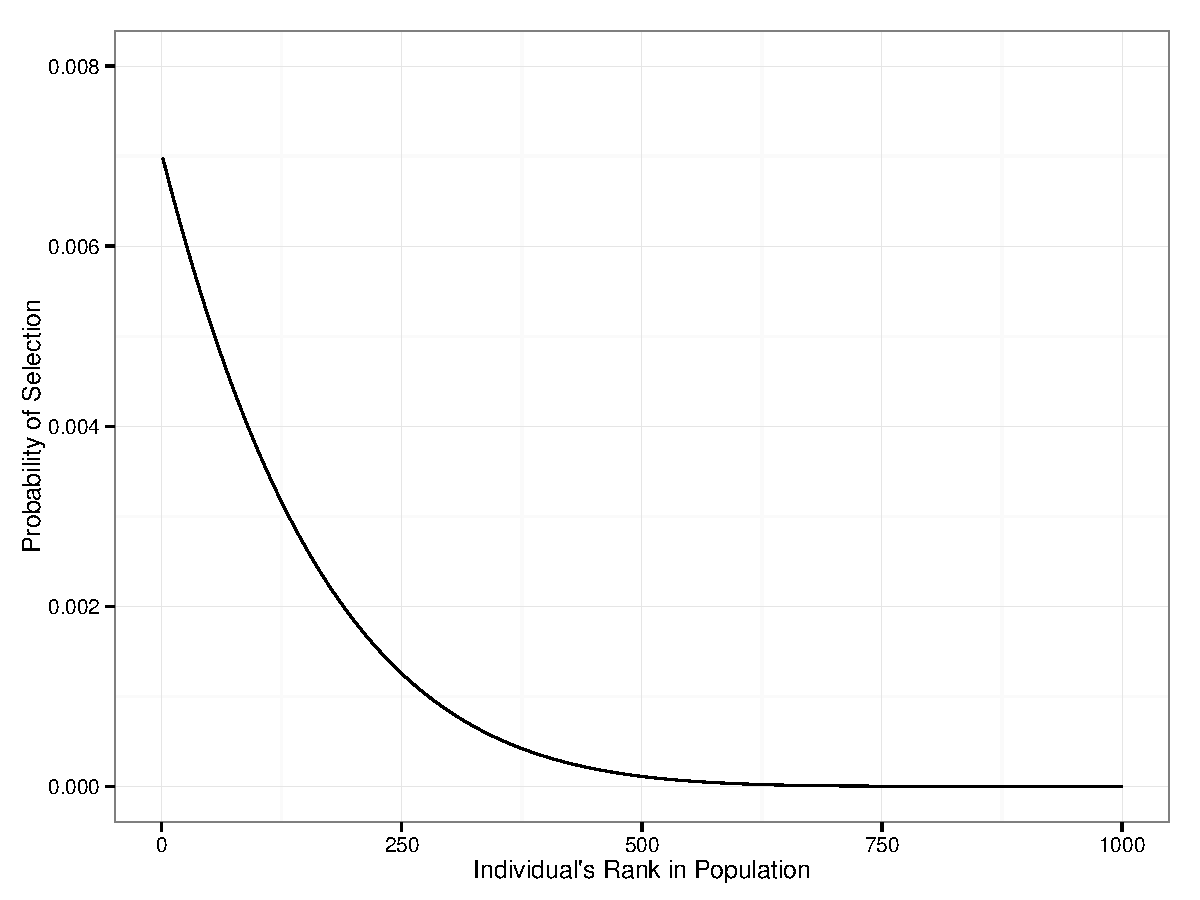
\includegraphics[width=\linewidth]{probSelectionTourney7.pdf}
\caption{Probability mass function of selecting individual with rank $i$ out of a population of 1000 individuals using tournament selection with tournament size 7, assuming no two individuals have the same rank. This plots Equation~\ref{tourneyProbEquation}.}
\label{fig:prob-selection-tourney-7}
\end{figure}

From Equation~\ref{tourneyProbEquation}, we see that in our runs using population size 1000 and tournament size 7, the best few individuals will be selected approximately 0.7\% of the time each. This also follows from the fact that every individual will participate in approximately 0.7\% of the tournaments, and the best individual will win each tournament in which it participates.
With tournament selection it would therefore be unlikely to hyperselect many individuals at the 1\% level in a generation, and extremely unlikely for any individuals to be hyper selected at the 5\% or 10\% level.
On the other hand, we have observed numerous examples of lexicase selection rewarding an interesting individual with over 90\% of the selections in a generation. We therefore expect lexicase selection to produce non-zero numbers of hyperselections at the 5\% and 10\% levels, though without empirical data it is unclear how common these will be.

\section{Experimental setup}
\label{section:experiments}

\todo[inline]{It's possible that lack of hyperselection is generally higher in successful runs. Can we easily split the numbers according to whether a run was successful or not? -- Nic

Tom: Done. Data is in Discourse. Do we want to report this at all? I'm ambivalent.
}

To empirically measure hyperselection, we gathered data from genetic programming runs using lexicase selection and tournament selection with size 7 tournaments. We tested each selection method on nine problems chosen from a recent general program synthesis benchmark suite~\cite{Helmuth:2015:GECCO}, a subset exhibiting a range of problem requirements and difficulties. We conducted 100 runs for each problem and parameter combination. We used PushGP \cite{spector:2002:GPEM, 1068292}, a stack-based genetic programming system, for these experiments since it supports a variety of control structures and multiple data types, making it a good choice for program synthesis tasks. Lexicase selection has also been shown to be effective in tree-based genetic programming \cite{Helmuth:2014:ieeeTEC, Krawiec:2015:GECCO:smgpWorkshop}.

We then calculated the average number of hyperselected individuals at the 1\%, 5\%, and 10\% levels per generation, which we present in the first three major columns of Table~\ref{table:slt-hyperselection}. On all problems except one, lexicase selection hyperselects 5 or more individuals per generation on average at the 1\% level; tournament selection averages less than one per generation on all problems, though always greater than 0.2. Unsurprisingly, tournament selection never hyperselected an individual at the 5\% or 10\% levels.
On 7 of the 9 problems, lexicase selection hyperselected one individual at the 5\% level in every 2 to 10 generations on average, and one individual at the 10\% level every 4 to 25 generations on average. 

The Vector Average and Count Odds problems showed much lower levels of hyperselection with lexicase selection, especially at the 5\% and 10\% levels, indicating that selecting a single individual to parent many of the children in a single generation was rarer on those problems. These two problems were also among the least-solved problems in this subset of the benchmark problems; one hypothesis is that most of the genetic programming runs had trouble getting any traction on these problems, leading to more homogeneous populations and fewer hyperselection events than on other problems.

\todo[inline]{We could probably check the hypothesis in the last sentence if we wanted to.

Tom: I'm not sure how we would do this. Any ideas Nic?
}

Considering that tournament selection conforms to the probability of selection given in Equation~\ref{tourneyProbEquation} regardless of problem, it is at first surprising that its hyperselections at the 1\% level vary as much as they do across problems. This difference is likely explained by how often tied individuals appear near the top of the rankings for different problems, since Equation~\ref{tourneyProbEquation} does not strictly hold in the presence of ties. Intuitively, if many individuals tie for the best rank, they will each win fewer tournaments than a single best individual would, since ties in tournaments are broken randomly. Therefore, lower hyperselection for tournament selection on a problem likely indicates that ties happened more often on those problems, which we have observed anecdotally in a few runs.

\todo[inline]{We could probably get data on the question in the last sentence if we wanted to.\\Tom: We could get some data, but it's not clear to me how we would present it. We'd have to do something like fit a regression line to "number of ties vs. hyper selections". Anyway, it all sounds too complicated to show a point that's nowhere close to our main goals. So, I say leave it as-is.}

The results in Table~\ref{table:slt-hyperselection} clearly show that lexicase selection gives more of its parent selections to single individuals than tournament selection, both at low levels (1\%) and higher levels (5\% and 10\%) of hyperselection. This indicates that lexicase selection more often concentrates its selection pressure on single individuals or small groups of individuals than tournament selection, increasing its exploitation of the individuals it selects most often. This data does not indicate whether lexicase selection is hyperselecting the same individuals that tournament selection ranks highest (those with best total error), or if it actually selects individuals that would receive few or no selections with tournament selection.

In Section \ref{section:lexicase} we referenced results that show genetic programming with lexicase selection significantly outperforms genetic programming with tournament selection across many benchmark problems. We have now observed that lexicase selection often concentrates selection pressure into small numbers of individuals. This raises important questions: can we attribute lexicase selection's success to its ability to concentrate selection in hyperselection events? Or, is it more important that lexicase selects different individuals than tournament selection, in some sense the ``right'' individuals to drive evolution toward a solution? We will investigate these questions in Section~\ref{section:HyperSelectionandLexicasePerformance}.

%-----------------------------------------------------------
%@@
% - Do I want to say something in this section, or in the other hyperselection section, about how large hyperselection events where a single individual "takes over" the population don't really seem to harm lexicase? Momentary blips of loss in diversity, but quickly regains that diversity.
\section{Hyperselection and Lexicase\\Performance}
\label{section:HyperSelectionandLexicasePerformance}

In Section~\ref{section:experiments} we saw that lexicase selection often ends up selecting the same individual many times in one generation, much more often than tournament selection does. This leads to the question of whether the hyperselections observed in lexicase selection runs are important in driving evolution toward solutions, or if they are simply a side effect of lexicase's algorithm. The alternative is that the individuals that lexicase selection selects the most often are simply different from those that tournament selection selects most often, in particular those with poor total error. In this section we test the hypothesis that the hyperselections we observed in runs using lexicase are integral to its success, and that without these extreme exploitative events, lexicase selection would perform significantly worse than it does with them.

To test this hypothesis, we designed a new parent selection algorithm that selects the same individuals most often that lexicase does, but has hyperselection characteristics much closer to tournament selection. The new algorithm, \definition{sampled lexicase-tournament selection} (SLT), starts by sampling the population, which only happens once per generation before selecting any parents. We sample $k$ individuals from the population by running the lexicase selection algorithm and tracking how often each individual is selected. In this work we set $k = 2P$, where $P$ is the population size (set to 1000 in our runs), guaranteeing at least as many samples as the number of parents that will be selected in that generation\footnote{We observe around 1700 parent selections per generation on average, which varies since we randomly select genetic operators, and some operators require one parent where others require two. This means that at most, 2000 parents could be selected in a generation.}. We then use the number of samples each individual received to rank the population from best (most samples) to worst (least samples). Next, every time we need to select a parent, we conduct a tournament, where the winner of the tournament is based on the lexicase-sampled ranking instead of total error. In this experiment we used size 7 tournaments, just like we did with tournament selection in our experiments.

SLT can be seen as a variation of tournament selection in which fitness is based on lexicase sampling instead of total error.
SLT gives the highest probabilities of selection to those individuals that lexicase would select the most often in the population. But, since it uses tournaments for selection, its probability of selecting the individual ranked $i$ in the lexicase-sampled ranking will be same as in tournament selection, as given in Equation~\ref{tourneyProbEquation}. Therefore, we would expect the hyperselection characteristics of SLT to mirror those of tournament selection, and differ only when the two behave differently with respect to tied individuals in the rankings, especially ties amongst the best individuals. To be clear, we developed SLT not because we believe it could be a useful parent selection method, but instead because it will allow us to test the hypothesis that hyperselection events are critical to lexicase selection's improved performance over tournament selection.

\begin{table*}[t]
\centering
\caption{
	The average number of hyperselected individuals at the 1\%, 5\%, and 10\% levels per generation for lexicase selection, tournament selection and SLT selection.
}
\label{table:slt-hyperselection}
\rowcolors{3}{white}{Gray}
\begin{tabu} to \textwidth {l | rrr | rrr | rrr}
\toprule
  & \multicolumn{3}{c|}{\textbf{Lexicase}} & \multicolumn{3}{c|}{\textbf{Tournament}} & \multicolumn{3}{c}{\textbf{SLT}} \\
\textbf{Problem} & \textbf{1\%}  & \textbf{5\%}  & \textbf{10\%}  & \textbf{1\%}      & \textbf{5\%}      & \textbf{10\%}   & \textbf{1\%}      & \textbf{5\%}      & \textbf{10\%}  \\
\midrule
Count Odds                 & 0.49  & 0.02 & 0.00 & 0.70 & 0.00 & 0.00 & 1.54 & 0.00 & 0.00 \\
Double Letters             & 12.28 & 0.29 & 0.09 & 0.36 & 0.00 & 0.00 & 1.54 & 0.00 & 0.00 \\
Mirror Image               & 9.72  & 0.23 & 0.05 & 0.22 & 0.00 & 0.00 & 1.55 & 0.00 & 0.00 \\
Negative To Zero           & 8.21  & 0.39 & 0.16 & 0.43 & 0.00 & 0.00 & 1.55 & 0.00 & 0.00 \\
Replace Space with Newline & 13.39 & 0.38 & 0.11 & 0.28 & 0.00 & 0.00 & 1.56 & 0.00 & 0.00 \\
String Lengths Backwards   & 6.21  & 0.54 & 0.25 & 0.42 & 0.00 & 0.00 & 1.53 & 0.00 & 0.00 \\
Syllables                  & 5.74  & 0.13 & 0.05 & 0.38 & 0.00 & 0.00 & 1.55 & 0.00 & 0.00 \\
Vector Average             & 6.99  & 0.02 & 0.01 & 0.91 & 0.00 & 0.00 & 1.56 & 0.00 & 0.00 \\
X-Word Lines               & 5.31  & 0.13 & 0.04 & 0.36 & 0.00 & 0.00 & 1.55 & 0.00 & 0.00 \\
\bottomrule
\end{tabu}
\end{table*}

We conducted 100 runs of PushGP using SLT on the same 9 benchmark problems; the hyperselection results for SLT are also included in Table~\ref{table:slt-hyperselection}. The first thing to note is that SLT has higher hyperselection at the 1\% level than tournament selection. Theoretically, we would expect SLT to behave similarly to tournament selection if neither had ties in rank within the population. We believe the differences we see here are a product of ties in total error when using tournament selection, especially near the top of the rankings. The relative consistency of SLT's 1\%-level hyperselection likely comes from the fact that it rarely had large numbers of tied individuals near the top of the rankings---we expect that tournament selection without ranking ties would also average around 1.55 hyperselections at the 1\% level per generation.

In these runs, SLT usually had lower hyperselection at the 1\% level than lexicase selection, and always lower at the 5\% and 10\% levels, on which it never had a non-zero result. Since SLT was designed to have similar hyperselection characteristics as tournament selection, it is unsurprising that it received no hyperselections at the upper levels. This means that SLT succeeds in our goal of creating a lexicase-based selection mechanism that never puts as much as 5\% of the parent selections in a generation on a single individual. This contrasts with lexicase selection, which often selects single individuals to make large numbers of the children for the next generation.

Since we have shown that SLT has similar hyperselection characteristics to tournament selection, let us now examine its performance results in these runs, which we present in Table~\ref{table:slt-results}. Across these 9 problems, SLT shows very similar performance to lexicase selection, and better performance than tournament selection on every problem. Both SLT and lexicase found at least one solution on each of the 9 problems, where tournament selection only found solutions to 6 of the problems. Comparing these methods using a chi-square test with the Holm correction, SLT never has a significantly different success rate compared to lexicase selection. SLT is significantly better than tournament selection on the same problems as lexicase except for Count Odds and X-Word Lines, on which it achieved fewer than the 8 successes necessary to be significantly better than tournament.
 SLT seems to slightly outperform lexicase selection on the easier problems where both find more solutions, and lexicase selection slightly outperforms SLT on the more difficult problems where both find fewer solutions, though the difference is never significant.

\begin{table}[t]
\centering
\caption{Number of successful runs out of 100 for each setting on each problem. For each problem, \underline{underline}~indicates significant improvement over tournament selection using a pairwise chi-squared test with Holm correction and 0.05 significance level. SLT and lexicase selection never have significantly different success rates.}
\label{table:slt-results}
\rowcolors{2}{Gray}{white}
\begin{tabular}{lrrr}
\toprule
\textbf{Problem}                    & \textbf{Lex} & \textbf{Tourn} & \textbf{SLT} \\
\midrule
Count Odds                 & \underline{8}        & 0          & 5   \\
Double Letters             & 6        & 0          & 4   \\
Mirror Image               & \underline{78}       & 46         & \underline{84}  \\
Negative To Zero           & \underline{45}       & 10         & \underline{53}  \\
Replace Space with Newline & \underline{51}       & 8          & \underline{61}  \\
String Lengths Backwards   & \underline{66}       & 7          & \underline{79}  \\
Syllables                  & \underline{18}       & 1          & \underline{13}  \\
Vector Average             & 16       & 14         & \underline{30}  \\
X-Word Lines               & \underline{8}        & 0          & 4   \\
\bottomrule
\end{tabular}
\end{table}

\todo[inline]{TOM IS CURRENTLY WORKING ON THE NEXT 2 ORANGE BUBBLES ABOUT DIVERSITY :D}

\todo[inline]{Should we just drop this next paragraph? -- Nic\\ Tom: I don't think so -- I think it's worth mentioning that the diversity is similar. If it were different, it could be a reason to prefer one or the other even though it didn't affect success rates on these problems, since different diversity might be important on other problems. In fact, if we have room, it might be worthwhile to insert one or two diversity plots here.
	
	Nic: There does seem to be room, so I'd be inclined to include them.}
We plotted the diversity across generations from the runs using SLT, as we did for other techniques in Section~\ref{section:exploration}. Interestingly, the diversity plots for SLT were virtually indistinguishable from those of lexicase selection, so we omit them here. Thus, even though the techniques produce significantly different hyperselection rates, their populations still maintain similar abilities to search widely.
\todo[inline]{Tom: We should tweak the above paragraph. One change should be to cite the lexicase paper and/or my dissertation where we show that lexicase leads to much higher diversity than tourney (and IFS). Or maybe that should be mentioned in the lexicase section?
	
	Nic: I added a (brief) mention of the diversity results (with a citation) in the Lexicase section. Is that enough, or should more be said?}

These results show that even though SLT has much lower hyperselection characteristics than lexicase selection, never selecting a single individual to parent more than 5\% of the children in a generation, it nevertheless maintains the problem-solving performance shown by lexicase selection. These results give strong evidence against the hypothesis that lexicase selection's increased exploitation of hyperselected individuals is important in its ability to outperform tournament selection with and without implicit fitness sharing. Instead, this suggests that it is more important \textit{which} individuals lexicase selection selects most often, which it has in common with SLT but not tournament selection.

While SLT achieved similar performance to lexicase selection in this experiment, it does not otherwise indicate that it would make a better parent selection mechanism. Notably, it will perform slightly slower than lexicase selection in practice, since it performs both lexicase sampling and then tournaments for selection. Even so, it may merit further examination on other types of problems to see if it behaves differently in other settings.


\section{Conclusions}
\label{section:conclusions}

Because lexicase selection can significantly improve the ability of genetic programming to solve hard problems, it would be useful to better understand the reasons that it sometimes works so well. Previous observations of the unusual phenomenon of hyperselection under lexicase selection, in which a single individual is selected as a parent in a very large number of selection events, suggested that there might be an interesting connection between hyperselection and the problem-solving power of lexicase selection.

The experiments presented here show that the problem-solving power of lexicase selection is maintained even if it is altered to prevent hyperselection, using selection frequencies like those of tournament selection (which we did with a selection method called ``sampled lexicase-tournament selection''). This means that the power of lexicase selection must stem from the collection of individuals that it tends to select, not from the unusual frequencies with which it sometimes selects them. Previous work had already shown that lexicase selection often selects specialist individuals that do well on some cases but poorly on others~\cite{Helmuth:2015:GPTP,Helmuth:2015:dissertation}, and our results here suggest that it may be the exploitation of these specialists that is primarily responsible for the unusual problem-solving power of lexicase selection.

One avenue for future research is to investigate the notion of a ``specialist'' more thoroughly, to determine if, perhaps, some kinds of specialists may be more valuable than others. 

Another is to investigate the connection between hyperselection and population diversity. Other work has shown that lexicase selection produces more diverse populations than tournament selection with or without implicit fitness sharing~\cite{Helmuth:2015:dissertation}, but we have not yet looked carefully at the diversity produced in the absence of hyperselection, as with sampled lexicase-tournament selection.

\todo[inline]{Tom: Have we observed differences in diversity? I forget. Say something about them being worth future study. Additionally, it seems that lexicase selection might be good at rediversifying the population after a hyperselection event.}
\todo[inline]{Tom: Here's a note I had about the above: Look at the hyperselected individuals, and what happens to the
population diversity in the first few generations afterward an
uber-hyperselection event. I think in run6 we saw rapid increases in
diversity after a valley, which would be interesting if that's the rule
rather than the outlier. It seems important that lexicase can escape the
un-diverse local optima quickly.}

\todo[inline]{Lee: Maybe not for this paper, but can lexicase selection be used for re-diversification even if it is not used otherwise? Might it be connected to speciation or quasi-Cambrian explosions?}



%ACKNOWLEDGMENTS are optional
\section{Acknowledgments}
Omitted for blind review.

%
% The following two commands are all you need in the
% initial runs of your .tex file to
% produce the bibliography for the citations in your paper.
\bibliographystyle{abbrv}
\bibliography{hyperbib}  % sigproc.bib is the name of the Bibliography in this case
% You must have a proper ".bib" file
%  and remember to run:
% latex bibtex latex latex
% to resolve all references
%
% ACM needs 'a single self-contained file'!
%
%APPENDICES are optional
%\balancecolumns

\end{document}
